\documentclass[10pt]{beamer}

\usepackage[english]{babel}
\usepackage[utf8]{inputenc}
\usepackage{amsmath,amssymb,amsthm,latexsym}
\usepackage{mathrsfs}
\usepackage[all]{xypic}
\usepackage{tikz}
\usetikzlibrary{arrows,matrix}
\usepackage{eurosym}
\usepackage{listings}
\usepackage{textcomp}
\usepackage{soul}

\usepackage[bibstyle=beamer,citestyle=authoryear-comp,doi=false,isbn=false,eprint=false,maxnames=10]{biblatex}
\bibliography{defeo}
\usepackage{mysymbols}


\newenvironment{pictureframe}{
  \addtocounter{framenumber}{-1}
  \setbeamertemplate{navigation symbols}{}
  \setbeamercolor{background canvas}{bg=black}
  \begin{frame}[plain,fragile,environment=pictureframe]%
    \begin{center}%
    }{%
    \end{center}%
  \end{frame}%
}

\lstset{
  upquote=true,
  basicstyle=\ttfamily,          % print whole listing in typewriter
  keywordstyle=\color{blue}\bfseries, % bold blue keywords
  %identifierstyle=,           % nothing happens
  commentstyle=\color{green}, % green comments
  stringstyle=\color{red},      % typewriter type for strings
  showstringspaces=false     % no special string spaces
}

\usepackage[amssymb,amsfonts]{concmath}
\renewcommand{\sfdefault}{uop}
\mode<presentation>{%
  \usetheme{Boadilla}
  \usefonttheme[onlymath]{serif}
  \usecolortheme[rgb={0.56,0.3,0}]{structure}
  \setbeamercolor{alerted text}{fg=blue}
}
\renewcommand{\emph}[1]{{\usebeamercolor[fg]{structure}#1}}


\title{Transposition principle and applications}
\author[Luca De Feo]{Luca De Feo\\\small{joint work with É. Schost and M. Boespflug}}
\institute{IRMAR}
\date{Rennes, April 1, 2011}


\begin{document}

\begin{frame}
  \titlepage
\end{frame}

%%
%%

\begin{frame}
  \frametitle{Or, ``The day I discovered I suffer from schizophrenia''}

  \begin{columns}[c]
    \begin{column}{0.5\textwidth}
      \begin{center}
        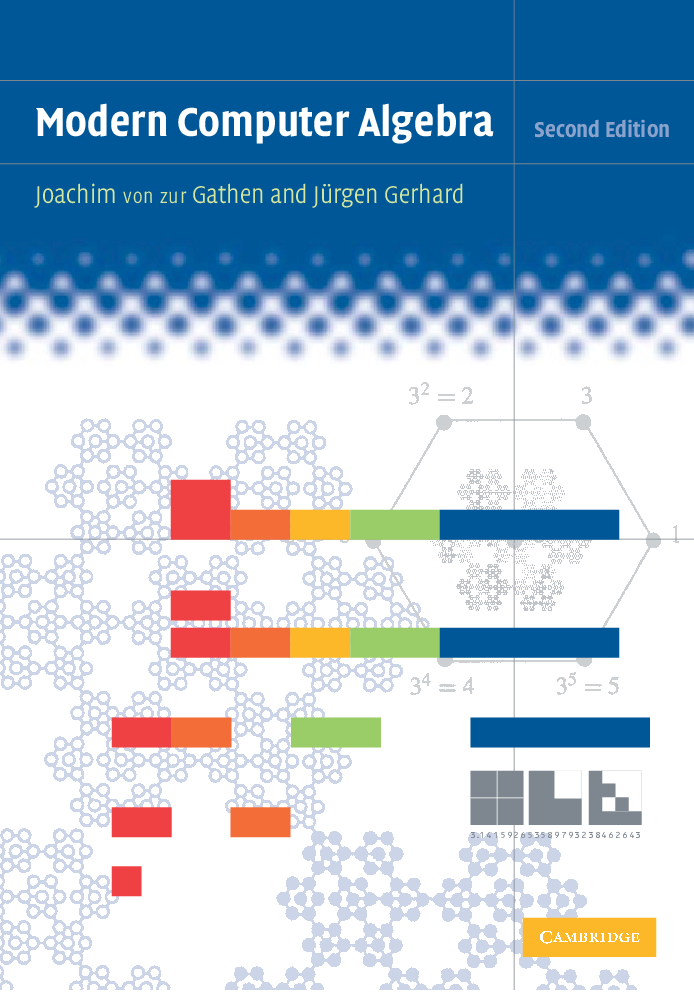
\includegraphics[width=0.8\textwidth]{modern.png}

        Dr. Jekyll is a computer algebraist
      \end{center}
    \end{column}
    \begin{column}{0.5\textwidth}
      \begin{center}
        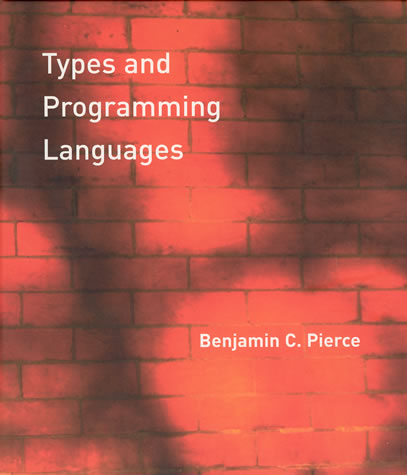
\includegraphics[width=0.8\textwidth]{types.jpg}
        
        Mr Type wastes precious research time reading about types and
        categorical semantics
      \end{center}
    \end{column}
  \end{columns}
\end{frame}

%%

\begin{pictureframe}
  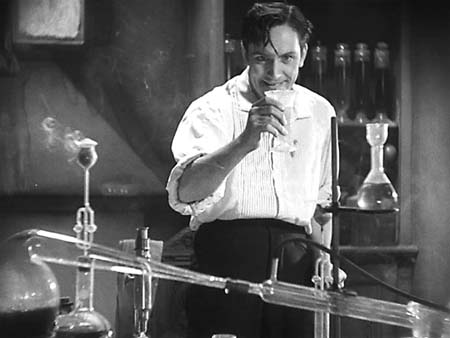
\includegraphics[width=\textwidth]{jekyll1}
\end{pictureframe}

%%
%%

\lstset{language=python}

\begin{frame}[fragile]
  \frametitle{Some trivialities}
  
  Suppose you have a computer program made \emph{exclusively} of
  ``steps'' in a given (Cartesian) category $\mathcal{C}$
  
  \begin{columns}
    \begin{column}{0.45\textwidth}
\begin{lstlisting}
  def foo(x in A,
          y in B)
    w = f(x, y)
    z = g(w, y)
    return z
\end{lstlisting}
    \end{column}
    \begin{column}{0.05\textwidth}
      \vfill
      \Large
      $\overset{F}{\Rightarrow}$
      \vfill
    \end{column}
    \begin{column}{0.5\textwidth}
\begin{lstlisting}
  def Ffoo(x in F(A),
           y in F(B))
    w = F(f)(x, y)
    z = F(g)(w, y)
    return z
\end{lstlisting}
    \end{column}
  \end{columns}

  Then, a functor $F:\mathcal{C}\to\mathcal{D}$ permits us to
  translate programs \emph{working in $\mathcal{C}$} into programs
  \emph{working in $\mathcal{D}$}.

  \begin{figure}
    \centering
    \begin{tikzpicture}
      \newcommand{\noF}[1]{#1}
      \newcommand{\yesF}[1]{\ensuremath F(#1)}

      \foreach \x/\y in {noF/0cm,yesF/6.5cm} {
        \def\apF{\csname \x \endcsname}
        \begin{scope}[xshift=\y]
          \matrix[matrix of math nodes,column sep=1em,row sep=2em,ampersand replacement=\&]{
            \& |(B)| \apF{B}           \& |(CxB)| \apF{C\times B} \& |(D)| \apF{D} \\
            |(A)| \apF{A} \& |(AxB)| \apF{A\times B} \& |(C)| \apF{C}\\
          };
          \scriptsize
          \path[right hook->] (A) edge (AxB);
          \path[right hook->] (B) edge (AxB);
          \path[->] (AxB) edge node[auto]{$\apF{f}$} (C);
          \path[right hook->] (B) edge (CxB);
          \path[right hook->] (C) edge (CxB);
          \path[->] (CxB) edge node[auto]{$\apF{g}$} (D);
        \end{scope}
      }
    \end{tikzpicture}
  \end{figure}

  This \emph{principle} is most useful when the functor is an
  \emph{equivalence of categories}.
\end{frame}

%%

\begin{frame}[fragile]
  \frametitle{Some more trivialities}
  
  \begin{block}{}
    If we measure the computational complexity of a program by its
    number of \emph{elementary steps}, this measure is invariant under
    equivalence of categories, provided the equivalence functor sends
    \emph{elementary arrows} in $\mathcal{C}$ to \emph{elementary
      arrows} in $\mathcal{D}$.

    \begin{figure}
      \centering
      \begin{tikzpicture}
        \newcommand{\noF}[1]{#1}
        \newcommand{\yesF}[1]{\ensuremath F(#1)}
        \newcommand{\noar}{->}
        \newcommand{\yesar}{<-}

        \foreach \x/\y in {no/0cm,yes/6.5cm} {
          \def\apF{\csname \x F\endcsname}
          \def\apar{\csname \x ar\endcsname}

          \begin{scope}[xshift=\y]
            \matrix[matrix of math nodes,column sep=1em,row sep=2em,ampersand replacement=\&]{
              |(A)| \apF{A} \& |(B)| \apF{B} \& |(C)| \apF{C}\\
              \& |(D)| \apF{D} \& |(E)| \apF{E}\\
            };
            \scriptsize
            \path[\apar] (A) edge (B);
            \path[\apar] (B) edge (C);
            \path[\apar] (C) edge (E);
            \path[\apar,red] (A) edge (D);
            \path[\apar,red] (D) edge (E);
          \end{scope}
          \pause
        }
      \end{tikzpicture}
    \end{figure}

    \begin{uncoverenv}<2->
      And it also works with contravariant functors (dualities)!
    \end{uncoverenv}
  \end{block}  
  
  \begin{block}{}<3-> For most of this talk, we'll be interested in
    the category of \emph{vector spaces} and we will look at the
    \emph{transposition functor} (which is not exactly an
    equivalence). Thus you can forget everything about categories and
    just keep in mind that
    \[\trans{(AB)} = \trans{B}\trans{A}.\]
  \end{block}
\end{frame}

%%

\begin{pictureframe}
  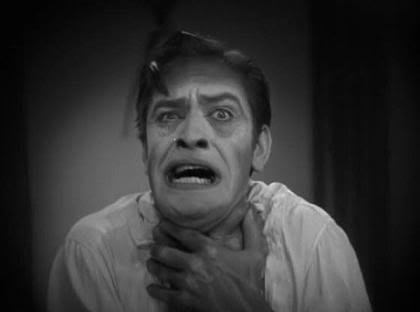
\includegraphics[width=\textwidth]{jekyll}
\end{pictureframe}


%%
%%

\begin{frame}
  \frametitle{Example: Middle product}

  \begin{block}{Newton iteration for the inverse of power series}
    \[G = 1/F \mod X^n, \qquad G + (1-GF)G = 1/F \mod X^{2n}.\]
    At each iteration,
    \[\deg G = n-1, \qquad \deg \left(F \bmod X^{2n}\right) = 2n-1, \qquad \deg GF = 3n-2,\]
    but \emph{$\quad X^n | (1-GF)\quad$} and \emph{$\quad\deg \left((1-GF)\bmod X^{2n}\right) = 2n-1$}.
  \end{block}
  
  \begin{equation*}
    GF = 
    \begin{pmatrix}
      g_0\\
      g_1 & g_0\\
      \hline
          & g_1 & g_0\\
          &     & g_1 & g_0\\
          \hline
          &     &     & g_1
    \end{pmatrix}
    \begin{pmatrix}
      f_0\\f_1\\f_2\\f_3
    \end{pmatrix}
    =
    \begin{pmatrix}
      1\\0\\\hline h_2\\h_3\\\hline h_4
    \end{pmatrix}
  \end{equation*}
\end{frame}

%%

\begin{frame}
  \frametitle{Example 1: Middle product}
  
  Set $\tilde{G} = X^nG(1/X) = g_0X^n + g_1X^{n-1} + \cdots + g_{n-1}X$, then
  \begin{equation*}
    \tilde{G}J =
    \begin{pmatrix}
      \\
      g_1\\
      g_0 & g_1\\
          & g_0
    \end{pmatrix}
    \begin{pmatrix}
      j_0\\j_1
    \end{pmatrix}
  \end{equation*}

  Hence \emph{$GF = X^n\trans{\tilde{G}}F  \bmod X^{2n}$}.

  \begin{block}{Complexity}
    \begin{itemize}
    \item The multiplication matrix of $\tilde{G}$ has $n^2$ non-zero
      coefficients: multiplying on the left or on the right costs
      $n^2$ multiplications plus $n(2n-1)$ additions by the row-column
      product. This is trivial and not very interesting.
    \item But we can compute $\tilde{G}J$ for any $J$ using only
      $\Mult(n)\in O(n\log n\loglog n)$ operations. The transposition
      principle says that we can compute $\trans{G}F$ for any $F$
      using \emph{exactly} the same number of operations.
    \item On the other hand, computing $GF$ and then extracting the
      coefficients of the middle costs about $\Mult(2n)$
      operations. This is \emph{worse} by a factor of $2$!
    \end{itemize}
  \end{block}
\end{frame}

%% 

\begin{frame}
  \frametitle{Arithmetic circuits}

  \begin{block}{Algebraic complexity}
    \centering Fix a field $\K$. We construct circuits that evaluate
    arithmetic functions.
  \end{block}


  \begin{center}
    Three gates: Addition, duplication, multiplication by a fixed
    element $a\in\K$.
    
    \begin{tikzpicture}
      \tikzstyle{node}=[circle,thick,draw=black,minimum size=4mm]
      
      \begin{scope}
        \node(in1){};
        \node(nop1)[right of=in1]{};
        \node(in2)[right of=nop1]{};
        \node(nop2)[right of=in2]{};
        \node(in3)[right of=nop2]{};
        \node(nop3)[right of=in3]{};
        \node(in4)[right of=nop3]{};
        
        \node[node](plus)[below of=nop1]{$+$}
        edge(in1)
        edge(in2);
        \node(nop)[below of=nop2]{};
        \node[node](hub)[below of=in3]{$\hub$}
        edge(in3);
        \node[node](times)[below of=in4]{$*_a$}
        edge(in4);
        
        \node(out1)[below of=plus]{}
        edge(plus);
        \node(nop5)[right of=out1]{};
        \node(out2)[below of=nop]{}
        edge(hub);
        \node(nop6)[below of=hub]{};
        \node(out3)[right of=nop6]{}
        edge(hub);
        \node(out4)[below of=times]{}
        edge(times);
      \end{scope}
    \end{tikzpicture}
  \end{center}
\end{frame}

%%

\begin{frame}
  \frametitle{Arithmetic circuits}

  \begin{columns}
    \begin{column}{0.6\textwidth}
      \centering
      \begin{tikzpicture}
        \tikzstyle{node}=[circle,thick,draw=black,minimum size=4mm]
        
        \begin{scope}
          \node(x1){$x_1$};
          \node(x2)[right of=x1]{$x_2$};
          \node(x3)[right of=x2]{$x_3$};
          
          \node[node](d1)[below of=x2]{$\hub$}
          edge(x2);
          \node[node](d2)[below of=x3]{$\hub$}
          edge(x3);
          
          \node[node](p1)[below of=d1,xshift=-6mm]{$+$}
          edge(x1)
          edge(d1);
          \node[node](m1)[below of=d2]{$*_3$}
          edge(d2);
          
          \node[node](p2)[below of=p1]{$+$}
          edge(p1)
          edge(d2);
          \node[node](p3)[right of=p2]{$+$}
          edge(d1)
          edge(m1);
          
          \node(y1)[below of=p2]{$y_1$}
          edge(p2);
          \node(y2)[below of=p3]{$y_2$}
          edge(p3);
        \end{scope}
      \end{tikzpicture}
    \end{column}
    \begin{column}{0.4\textwidth}
      \begin{align*}
        y_1 &= x_1 + x_2 + x_3\\
        y_2 &= x_2 + 3x_3
      \end{align*}
      
      \Large
      \begin{gather*}
        \begin{pmatrix}
          1 & 1 & 1\\
          0 & 1 & 3
        \end{pmatrix}
      \end{gather*}
    \end{column}
  \end{columns}
\end{frame}

%%

\begin{frame}
  \frametitle{Transposition of an arithmetic circuit}

  \begin{columns}
    \begin{column}{0.6\textwidth}
      \centering
      \begin{tikzpicture}
        \tikzstyle{node}=[circle,thick,draw=black,minimum size=4mm]
        
        \begin{scope}
          \node(x1){$x_1$};
          \node(x2)[right of=x1]{$x_2$};
          \node(x3)[right of=x2]{$x_3$};
          
          \node[node](d1)[below of=x2]{$\hub$}
          edge(x2);
          \node[node](d2)[below of=x3]{$\hub$}
          edge(x3);
            
          \node[node](p1)[below of=d1,xshift=-6mm]{$+$}
          edge(x1)
          edge(d1);
          \node[node](m1)[below of=d2]{$*_3$}
          edge(d2);
          
          \node[node](p2)[below of=p1]{$+$}
          edge(p1)
          edge(d2);
          \node[node](p3)[right of=p2]{$+$}
          edge(d1)
          edge(m1);
          
          \node(y1)[below of=p2]{$y_1$}
          edge(p2);
          \node(y2)[below of=p3]{$y_2$}
          edge(p3);
        \end{scope}
        
        \begin{scope}[xshift=3.2cm, yshift=-0.23\textheight]
          \node(x){\Huge $\leftrightarrow$};
        \end{scope}
        
        \begin{scope}[xshift=4cm, yshift=-0.425\textheight]
          \node(x1){$x_1'$};
          \node(x2)[right of=x1]{$x_2'$};
          \node(x3)[right of=x2]{$x_3'$};
          
          \node[node](d1)[above of=x2]{\alt<2>{$+$}{$\hub$}}
          edge(x2);
          \node[node](d2)[above of=x3]{\alt<2>{$+$}{$\hub$}}
          edge(x3);
          
          \node[node](p1)[above of=d1,xshift=-5mm]{\alt<2>{$\hub$}{$+$}}
          edge(x1)
          edge(d1);
          \node[node](m1)[above of=d2]{$*_3$}
          edge(d2);
          
          \node[node](p2)[above of=p1]{\alt<2>{$\hub$}{$+$}}
          edge(p1)
          edge(d2);
          \node[node](p3)[right of=p2]{\alt<2>{$\hub$}{$+$}}
          edge(d1)
          edge(m1);
          
          \node(y1)[above of=p2]{$y_1'$}
          edge(p2);
          \node(y2)[above of=p3]{$y_2'$}
          edge(p3);
        \end{scope}
      \end{tikzpicture}
    \end{column}
    \begin{column}{0.4\textwidth}
      \begin{align*}
        y_1 &= x_1 + x_2 + x_3\\
        y_2 &= x_2 + 3x_3
      \end{align*}
      
      \Large
      \begin{gather*}
        \begin{pmatrix}
          1 & 1 & 1\\
          0 & 1 & 3
        \end{pmatrix}\\
        \updownarrow\\
        \begin{pmatrix}
          1 & 0\\
          1 & 1\\
          1 & 3\\
        \end{pmatrix}
      \end{gather*}
    \end{column}
  \end{columns}
\end{frame}

%%

\begin{frame}
  \frametitle{Arithmetic Circuits: uniform vs. non-uniform}

  \begin{definition}[Circuit family]
    A \emph{circuit family} is a family $(C_0,C_1,\ldots)$ of circuits
    indexed by $\N$ such that $C_n$ has $n$ inputs.
  \end{definition}
  
  \begin{itemize}
  \item This gives the usual notion of complexity as a mapping
    $\N\to\N$.
  \item \alert{Any Turing-undecidable problem has a trivial
      \emph{polynomial-size} circuit family deciding it.}
  \end{itemize}

  \begin{definition}[Uniform circuit family]
    A circuit family $(C_0,C_1,\ldots)$ is said to be \emph{uniform}
    if there is a $\log n$-space bounded touring machine which on
    input $1^n$ outputs a representation of $C_n$.
  \end{definition}

  \begin{itemize}
  \item The transposition principle preserves uniformity.
  \item However, notice that there is no consistent way of analysing
    \emph{space complexity} in this model.
  \end{itemize}
\end{frame}

%%

\begin{frame}
  \frametitle{Vandermonde matrices}

  Let $P$ be a degree $n$ polynomial and let $a_1,\ldots,a_m$ be
  evaluation points, then
  \begin{equation*}
    V_{a_1,\ldots,a_m}P =
    \begin{pmatrix}
      1 & a_1 & \cdots & a_1^n\\
      \vdots & \vdots & & \vdots\\
      1 & a_m & \cdots & a_m^n
    \end{pmatrix}
    \begin{pmatrix}
      p_0\\p_1\\\vdots\\p_n
    \end{pmatrix}
    =
    \begin{pmatrix}
      P(a_1)\\\vdots\\P(a_m)
    \end{pmatrix}
  \end{equation*}
  where $V_{a_1,\ldots,a_m}$ is a Vandermonde matrix, the transposed
  problem is known as \emph{weighted Newton sums}.

  \begin{block}{Applications of the transposition principle}
    \begin{itemize}
    \item Solving sparse polynomial systems
      \parencite{canny+kaltofen+yagati89};
    \item Improving the complexity of multipoint evaluation;
    \item Equivalence between the complexities of interpolation and
      multipoint evaluation \parencite{bostan+schost04}.
    \end{itemize}
  \end{block}
\end{frame}

%%

\begin{frame}
  \frametitle{Transposed modular multiplication}
  
\end{frame}

%%

\begin{frame}
  \frametitle{Polynomial evaluation}
  
\end{frame}

%%

\begin{frame}
  \frametitle{Automatic differentiation}
  
\end{frame}

%%
%%

\begin{pictureframe}
  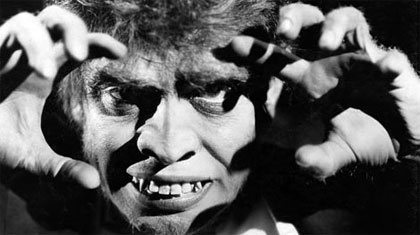
\includegraphics[width=\textwidth]{hyde2}
\end{pictureframe}

%%

\begin{frame}
  \frametitle{Automatic transposition}
  
\end{frame}

%%
%%

{
  \setbeamertemplate{navigation symbols}{}
  \setbeamertemplate{background canvas}{
\includegraphics[width=\paperwidth]{hyde}}
  \begin{frame}[plain]
    \vspace{8cm}
    \begin{center}
      \textcolor{white}{\Huge The End?}
    \end{center}
  \end{frame}
}

%%
%%

\end{document}




%%% Local Variables: 
%%% mode:flyspell
%%% ispell-local-dictionary:"american"
%%% mode: TeX-PDF
%%% TeX-master: t
%%% End: 
%
% LocalWords:  Tellegen
